\section{Tổng quan về nền tảng Nordic}
\label{sec:nordic}

Nordic Semiconductor là một trong những công ty hàng đầu thế giới trong lĩnh vực thiết kế và sản xuất các giải pháp truyền thông không dây công suất thấp (Ultra Low Power Wireless). Được thành lập năm 1983 tại Trondheim, Na Uy, Nordic đã phát triển thành một trong những nhà cung cấp chip wireless hàng đầu với hơn 40 năm kinh nghiệm trong ngành công nghiệp bán dẫn.

Các sản phẩm của Nordic được sử dụng rộng rãi trong nhiều lĩnh vực ứng dụng đa dạng, từ các thiết bị IoT như cảm biến thông minh và thiết bị theo dõi tài sản, đến các thiết bị đeo thông minh (wearables) như đồng hồ thông minh, vòng đeo tay sức khỏe và tai nghe không dây. Trong lĩnh vực smart home, chip của Nordic được tích hợp trong các thiết bị điều khiển ánh sáng, khóa cửa thông minh, và các hệ thống tự động hóa nhà ở. Đặc biệt, với khả năng tiêu thụ năng lượng cực thấp và hỗ trợ đa giao thức truyền thông, các sản phẩm của Nordic rất phù hợp cho việc triển khai các mạng cảm biến không dây ad-hoc - nơi các node cần hoạt động độc lập trong thời gian dài với nguồn pin hạn chế.

Điểm mạnh cốt lõi của Nordic nằm ở việc tích hợp hoàn chỉnh giữa phần cứng RF hiệu suất cao với bộ xử lý ARM tiên tiến trong một System-on-Chip (SoC) đơn nhất. Cách tiếp cận này giúp giảm thiểu kích thước bo mạch, đơn giản hóa thiết kế phần cứng, và tối ưu hóa chi phí sản xuất cho các nhà phát triển sản phẩm. Bên cạnh đó, Nordic còn cung cấp một hệ sinh thái phát triển phần mềm hoàn chỉnh bao gồm SDK, công cụ debug, và tài liệu kỹ thuật chi tiết, giúp rút ngắn đáng kể thời gian đưa sản phẩm ra thị trường.

\subsection{Vi điều khiển nRF54L15 series}

nRF54L15 là thế hệ System-on-Chip (SoC) mới nhất thuộc dòng nRF54L Series của Nordic, được thiết kế để thay thế dòng nRF52 với hiệu năng cao hơn và tiêu thụ năng lượng thấp hơn. Chip này tích hợp bộ xử lý ARM Cortex-M33 với các tính năng bảo mật tiên tiến và khả năng truyền thông không dây đa giao thức.

\begin{table}[h!]
\centering
\caption{Thông số kỹ thuật của nRF54L15}
\label{tab:nrf54l15_specs}
\begin{tabular}{|l|l|}
\hline
\textbf{Thông số} & \textbf{Giá trị} \\
\hline
CPU chính & ARM Cortex-M33 @ 128 MHz \\
\hline
CPU phụ (FLPR) & RISC-V @ 128 MHz \\
\hline
Flash & 1.5 MB \\
\hline
RAM & 256 KB \\
\hline
Bluetooth & LE 5.4 (LE Audio, Direction Finding) \\
\hline
IEEE 802.15.4 & Có (Thread, Zigbee, Matter) \\
\hline
Proprietary 2.4 GHz & Có (ESB compatible) \\
\hline
Công suất TX & -20 dBm đến +8 dBm \\
\hline
Độ nhạy RX & -98 dBm (BLE 1 Mbps) \\
\hline
Dải nhiệt độ & -40°C đến +105°C \\
\hline
Nguồn cấp & 1.7V - 3.6V \\
\hline
Bảo mật & ARM TrustZone, Secure boot, KMU \\
\hline
\end{tabular}
\end{table}

\subsubsection{Kiến trúc bộ xử lý}

nRF54L15 sử dụng kiến trúc dual-core độc đáo với sự kết hợp giữa ARM Cortex-M33 và RISC-V:

\textbf{CPU chính - ARM Cortex-M33:}
\begin{itemize}
    \item Tần số hoạt động tối đa 128 MHz, gấp đôi so với Cortex-M4 @ 64 MHz của nRF52840.
    \item Hỗ trợ DSP (Digital Signal Processing) extension cho các tác vụ xử lý tín hiệu số như lọc, FFT, và xử lý âm thanh.
    \item Tích hợp FPU (Floating Point Unit) đơn chính xác, tăng tốc các phép tính số thực trong thuật toán định vị và điều khiển.
    \item Kiến trúc ARMv8-M với TrustZone-M, cho phép phân chia phần cứng thành vùng Secure và Non-secure, đảm bảo an toàn cho các ứng dụng nhạy cảm.
    \item Pipeline 3 giai đoạn với branch prediction, giảm thiểu stall và tăng throughput.
\end{itemize}

\textbf{CPU phụ - RISC-V FLPR (Fast Lightweight Peripheral Processor):}
\begin{itemize}
    \item Bộ xử lý RISC-V 32-bit chạy ở tần số 128 MHz, hoạt động độc lập với CPU chính.
    \item Được thiết kế đặc biệt cho các tác vụ real-time yêu cầu độ trễ thấp như xử lý GPIO, giao tiếp SPI/I2C tốc độ cao, và các protocol timing-critical.
    \item Có thể hoạt động trong khi CPU chính ở chế độ sleep, tiết kiệm năng lượng đáng kể cho các ứng dụng cần phản hồi nhanh nhưng không yêu cầu xử lý phức tạp.
    \item Chia sẻ bộ nhớ với CPU chính thông qua cơ chế inter-processor communication (IPC).
    \item Đặc biệt hữu ích trong các ứng dụng mạng ad-hoc, nơi FLPR có thể xử lý các tác vụ định tuyến và quản lý gói tin mà không làm gián đoạn CPU chính.
\end{itemize}

\begin{figure}[h!]
    \centering
    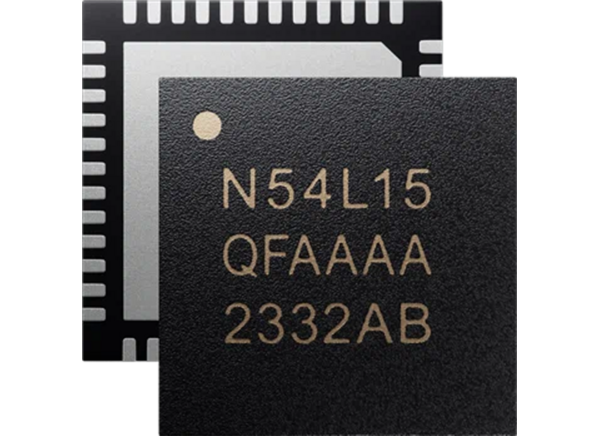
\includegraphics[width=1\textwidth]{chapter3/image/nRF54L15.png}
    \caption{Vi điều khiển nRF54L15}
    \label{fig:nrf54l15}
\end{figure}

\subsubsection{Hệ thống bộ nhớ}

nRF54L15 được trang bị hệ thống bộ nhớ mạnh mẽ, đáp ứng yêu cầu của các ứng dụng phức tạp:

\textbf{Flash Memory - 1.5 MB:}
\begin{itemize}
    \item Dung lượng lớn cho phép lưu trữ firmware phức tạp, nhiều giao thức wireless, và dữ liệu cấu hình.
    \item Hỗ trợ Execute-in-Place (XiP), cho phép chạy code trực tiếp từ Flash mà không cần copy vào RAM.
    \item Tích hợp cơ chế wear-leveling để kéo dài tuổi thọ Flash trong các ứng dụng ghi dữ liệu thường xuyên.
    \item Có thể phân vùng linh hoạt cho bootloader, application, và storage.
\end{itemize}

\textbf{RAM - 256 KB:}
\begin{itemize}
    \item Đủ dung lượng cho stack BLE Mesh, bảng định tuyến gradient, và buffer dữ liệu.
    \item Hỗ trợ retention mode trong sleep, cho phép lưu trữ trạng thái mà không mất dữ liệu.
    \item Có thể cấu hình selective retention để chỉ giữ một phần RAM, giảm thiểu dòng tiêu thụ.
\end{itemize}

\subsubsection{Khối Radio 2.4 GHz}

Khối Radio của nRF54L15 là một trong những điểm mạnh nhất của chip, hỗ trợ đa giao thức trên cùng một phần cứng:

\textbf{Bluetooth Low Energy 5.4:}
\begin{itemize}
    \item Hỗ trợ đầy đủ các tính năng BLE 5.4 bao gồm LE Audio (LC3 codec), Direction Finding (AoA/AoD), và Periodic Advertising with Responses (PAwR).
    \item Throughput tối đa 2 Mbps với LE 2M PHY, hoặc range mở rộng với LE Coded PHY (125 kbps / 500 kbps).
    \item Hỗ trợ Bluetooth Mesh theo chuẩn Mesh Profile 1.1, cho phép xây dựng mạng mesh với hàng nghìn node.
    \item Advertising extension cho phép gửi payload lên đến 255 bytes trong một packet.
\end{itemize}

\textbf{IEEE 802.15.4:}
\begin{itemize}
    \item Hỗ trợ đầy đủ chuẩn IEEE 802.15.4-2015 với tốc độ 250 kbps.
    \item Tương thích với các giao thức Thread, Zigbee, và Matter.
    \item Hỗ trợ CSL (Coordinated Sampled Listening) và TSCH (Time-Slotted Channel Hopping) cho các ứng dụng tiết kiệm năng lượng.
\end{itemize}

\textbf{Proprietary 2.4 GHz:}
\begin{itemize}
    \item Tương thích với giao thức ESB (Enhanced ShockBurst) của các dòng nRF trước.
    \item Hỗ trợ tốc độ 1 Mbps và 2 Mbps với độ trễ cực thấp (< 1 ms).
    \item Cho phép thiết kế giao thức tùy chỉnh với toàn quyền kiểm soát timing và packet format.
\end{itemize}

\textbf{Thông số RF:}
\begin{itemize}
    \item Công suất phát: -20 dBm đến +8 dBm (có thể điều chỉnh theo từng bước 1 dB).
    \item Độ nhạy thu: -98 dBm (BLE 1 Mbps), -103 dBm (BLE Coded 125 kbps).
    \item Dải tần số: 2400 MHz - 2483.5 MHz (ISM band).
    \item Hỗ trợ antenna diversity để cải thiện chất lượng liên kết trong môi trường multipath.
\end{itemize}

\subsubsection{Hệ thống bảo mật}

nRF54L15 tích hợp hệ thống bảo mật toàn diện, đáp ứng yêu cầu của các ứng dụng IoT hiện đại:

\textbf{Trusted Firmware-M:}
\begin{itemize}
    \item Phân chia phần cứng thành vùng Secure và Non-secure ở mức hardware.
    \item Secure code có thể truy cập tất cả tài nguyên, trong khi Non-secure code bị giới hạn.
    \item Cho phép lưu trữ khóa mật mã và thực hiện các phép toán nhạy cảm trong vùng Secure.
\end{itemize}

\textbf{CRACEN (Crypto Accelerator Engine):}
\begin{itemize}
    \item Hardware accelerator cho các thuật toán mã hóa phổ biến.
    \item AES-128/192/256 với các chế độ ECB, CBC, CTR, CCM, GCM.
    \item SHA-256, SHA-384, SHA-512 cho hash và HMAC.
    \item ECC (Elliptic Curve Cryptography) với các đường cong P-256, P-384.
    \item RSA với key size lên đến 4096 bits.
    \item Tốc độ xử lý cao hơn nhiều lần so với software implementation.
\end{itemize}

\textbf{Key Management Unit (KMU):}
\begin{itemize}
    \item Lưu trữ an toàn các khóa mật mã trong hardware.
    \item Khóa không thể đọc ra bằng software, chỉ có thể sử dụng cho các phép toán crypto.
    \item Hỗ trợ key derivation và key wrapping.
\end{itemize}

\textbf{Secure Boot:}
\begin{itemize}
    \item Xác thực firmware trước khi chạy, ngăn chặn firmware giả mạo.
    \item Chain of trust từ ROM bootloader đến application.
    \item Hỗ trợ firmware update an toàn (FOTA - Firmware Over The Air).
\end{itemize}

\subsubsection{Peripheral và I/O}

Vi điều khiển nRF54L15 có peripheral phong phú cho các ứng dụng đa dạng như trong bảng \ref{tab:nrf54l15_peripherals} dưới đây:

\begin{table}[h!]
\centering
\caption{Các peripheral của nRF54L15}
\label{tab:nrf54l15_peripherals}
\begin{tabular}{|l|l|}
\hline
\textbf{Peripheral} & \textbf{Đặc điểm} \\
\hline
GPIO & 32 pins, có thể cấu hình input/output, interrupt \\
\hline
UART & 2 instances, tốc độ lên đến 1 Mbps \\
\hline
SPI & 3 instances, master/slave, tốc độ lên đến 32 MHz \\
\hline
I2C (TWI) & 2 instances, tốc độ 100/400 kHz, hỗ trợ DMA \\
\hline
PWM & 3 instances, 4 channels mỗi instance \\
\hline
ADC (SAADC) & 12-bit, 8 channels, 200 ksps \\
\hline
Timer & 3 instances 32-bit, 1 RTC \\
\hline
Comparator & Low-power analog comparator \\
\hline
Temperature Sensor & On-chip, độ chính xác ±2°C \\
\hline
\end{tabular}
\end{table}

\subsubsection{Thông số năng lượng}

Tiêu thụ năng lượng là một trong những ưu điểm nổi bật nhất của nRF54L15. Theo datasheet chính thức của Nordic Semiconductor \cite{nordic_nrf54l15_ps}, chip này đạt được hiệu suất năng lượng vượt trội so với các thế hệ trước:

\begin{table}[h!]
\centering
\caption{Thông số tiêu thụ năng lượng của nRF54L15}
\label{tab:nrf54l15_power}
\begin{tabular}{|l|l|}
\hline
\textbf{Chế độ hoạt động} & \textbf{Dòng tiêu thụ} \\
\hline
System OFF (no RAM retention) & 0.3 $\mu$A \\
\hline
System OFF (full RAM retention) & 1.0 $\mu$A \\
\hline
System ON (idle, LFCLK running) & 2.5 $\mu$A \\
\hline
CPU active (từ Flash) & 30 $\mu$A/MHz \\
\hline
CPU active (từ RAM) & 25 $\mu$A/MHz \\
\hline
Radio TX (+0 dBm) & 3.8 mA \\
\hline
Radio TX (+8 dBm) & 8.5 mA \\
\hline
Radio RX & 3.2 mA \\
\hline
FLPR active & 10 $\mu$A/MHz \\
\hline
\end{tabular}
\end{table}

Ước tính thời gian hoạt động: Với các thông số trên, một node mạng ad-hoc sử dụng nRF54L15 với pin CR2032 (225 mAh) có thể hoạt động trong thời gian dài nếu được thiết kế duty cycle hợp lý. Ví dụ, với duty cycle 1\% (wake up 10 ms mỗi giây để kiểm tra message), dòng tiêu thụ trung bình chỉ khoảng 40 $\mu$A, cho phép thời gian hoạt động lên đến 5000 giờ (khoảng 7 tháng). Đây là ưu điểm quan trọng cho các ứng dụng mạng cảm biến ad-hoc, nơi các node thường hoạt động độc lập với nguồn pin hạn chế.


\subsubsection{So sánh với các dòng chip trước}

Bảng \ref{tab:nrf_comparison} so sánh nRF54L15 với các dòng chip Nordic phổ biến khác:

\begin{table}[h!]
\centering
\caption{So sánh nRF54L15 với các dòng chip Nordic khác}
\label{tab:nrf_comparison}
\begin{tabular}{|l|c|c|c|c|}
\hline
\textbf{Đặc điểm} & \textbf{nRF52832} & \textbf{nRF52840} & \textbf{nRF5340} & \textbf{nRF54L15} \\
\hline
CPU & M4 @ 64 MHz & M4 @ 64 MHz & M33 @ 128 MHz & M33 @ 128 MHz \\
\hline
Co-processor & Không & Không & M33 @ 64 MHz & RISC-V @ 128 MHz \\
\hline
Flash & 512 KB & 1 MB & 1 MB + 256 KB & 1.5 MB \\
\hline
RAM & 64 KB & 256 KB & 512 KB + 64 KB & 256 KB \\
\hline
BLE & 5.0 & 5.0 & 5.3 & 5.4 \\
\hline
802.15.4 & Không & Có & Có & Có \\
\hline
TrustZone & Không & Không & Có & Có \\
\hline
TX current & 5.3 mA & 4.8 mA & 3.2 mA & 3.8 mA \\
\hline
RX current & 5.4 mA & 4.6 mA & 2.9 mA & 3.2 mA \\
\hline
\end{tabular}
\end{table}

Từ bảng so sánh có thể thấy nRF54L15 mang lại sự cân bằng tốt giữa hiệu năng, tính năng, và tiêu thụ năng lượng. So với nRF52840 - dòng chip phổ biến nhất hiện nay, nRF54L15 có hiệu năng CPU gấp đôi, hỗ trợ BLE 5.4 mới nhất, có bộ xử lý phụ RISC-V linh hoạt, và tích hợp bảo mật TrustZone. Những cải tiến này làm cho nRF54L15 trở thành lựa chọn lý tưởng cho các ứng dụng mạng ad-hoc và IoT thế hệ mới.

\subsection{Môi trường phát triển}

Nordic Semiconductor cung cấp một hệ sinh thái phát triển phần mềm hoàn chỉnh và chuyên nghiệp cho dòng chip nRF54L15, giúp các nhà phát triển có thể nhanh chóng xây dựng và triển khai các ứng dụng IoT phức tạp. Hệ sinh thái này bao gồm bộ SDK mạnh mẽ, các công cụ phát triển tích hợp, và kit phần cứng hỗ trợ debug toàn diện.

\subsubsection{nRF Connect SDK}

nRF Connect SDK là bộ Software Development Kit chính thức của Nordic dành cho các dòng chip nRF52, nRF53, và nRF54. Đây là một bộ SDK thế hệ mới được xây dựng trên nền tảng Zephyr RTOS - một hệ điều hành thời gian thực mã nguồn mở được quản lý bởi Linux Foundation. Việc sử dụng Zephyr làm nền tảng mang lại nhiều lợi ích quan trọng: thứ nhất, Zephyr có cộng đồng phát triển lớn với hàng nghìn contributor từ các công ty công nghệ hàng đầu như Intel, Google, Facebook, và Nordic; thứ hai, Zephyr được thiết kế với kiến trúc modular cho phép tùy chỉnh linh hoạt theo yêu cầu của từng ứng dụng; thứ ba, Zephyr hỗ trợ đa dạng các kiến trúc vi xử lý từ ARM Cortex-M đến RISC-V, giúp code có tính portable cao.

Về mặt giao thức truyền thông, nRF Connect SDK cung cấp implementation đầy đủ và được chứng nhận cho các giao thức wireless phổ biến. Đối với Bluetooth Low Energy, SDK hỗ trợ toàn bộ các tính năng của BLE 5.4 bao gồm LE Audio với codec LC3, Direction Finding cho các ứng dụng định vị trong nhà (indoor positioning), Periodic Advertising with Responses (PAwR) cho các ứng dụng Electronic Shelf Label (ESL), và đặc biệt là Bluetooth Mesh theo chuẩn Mesh Protocol 1.1. Đối với các ứng dụng smart home và industrial IoT, SDK cung cấp stack Thread và Zigbee hoàn chỉnh, cùng với hỗ trợ cho giao thức Matter - chuẩn thống nhất mới cho các thiết bị smart home được phát triển bởi Connectivity Standards Alliance với sự tham gia của Apple, Google, Amazon, và Samsung.

Bên cạnh các giao thức truyền thông, nRF Connect SDK còn tích hợp đầy đủ driver và Hardware Abstraction Layer (HAL) cho tất cả các peripheral của nRF54L15. Các driver này được tối ưu hóa để tận dụng tối đa các tính năng phần cứng như DMA, PPI (Programmable Peripheral Interconnect), và các chế độ tiết kiệm năng lượng. SDK cũng cung cấp thư viện mật mã phần cứng để tương tác với CRACEN crypto accelerator, cho phép thực hiện các phép toán mã hóa AES, SHA, ECC với tốc độ cao và tiêu thụ năng lượng thấp hơn nhiều so với implementation bằng software.

Một điểm mạnh quan trọng khác của nRF Connect SDK là hỗ trợ toàn diện cho ARM TrustZone-M trên nRF54L15. SDK cung cấp Trusted Firmware-M (TF-M) làm secure firmware, cho phép phát triển các ứng dụng với mô hình bảo mật phân tầng: code nhạy cảm như xử lý khóa mật mã và xác thực được chạy trong Secure Processing Environment (SPE), trong khi application code chạy trong Non-Secure Processing Environment (NSPE). Mô hình này đảm bảo rằng ngay cả khi application code bị compromise, các tài nguyên bảo mật vẫn được bảo vệ.

\subsubsection{Công cụ phát triển tích hợp}

Nordic cung cấp bộ công cụ nRF Connect for Visual Studio Code như môi trường phát triển tích hợp (IDE) chính thức cho nRF Connect SDK. Extension này biến VS Code - một trong những code editor phổ biến nhất hiện nay - thành một IDE đầy đủ tính năng cho phát triển embedded. nRF Connect for VS Code tích hợp chặt chẽ với hệ thống build CMake và West (công cụ meta-build của Zephyr), cho phép cấu hình project, chọn board target, và build firmware chỉ với vài click chuột. Extension cũng cung cấp giao diện trực quan cho việc cấu hình Kconfig - hệ thống configuration của Zephyr, giúp developer dễ dàng enable/disable các tính năng và tùy chỉnh các tham số hệ thống mà không cần chỉnh sửa file cấu hình thủ công.

Về khả năng debug, nRF Connect for VS Code hỗ trợ đầy đủ các tính năng debug thông qua J-Link debugger tích hợp trên các Development Kit của Nordic hoặc các debugger external. Developer có thể đặt breakpoint, step through code, inspect variables, và xem call stack trực tiếp trong VS Code. Extension còn tích hợp với SEGGER RTT (Real-Time Transfer) để hiển thị log output từ device với độ trễ cực thấp, và với SEGGER SystemView để visualize hoạt động của RTOS bao gồm task scheduling, interrupt handling, và resource usage.

Song song với VS Code extension, Nordic còn cung cấp bộ công cụ nRF Connect for Desktop - một ứng dụng desktop đa nền tảng (Windows, macOS, Linux) với giao diện đồ họa thân thiện. nRF Connect for Desktop bao gồm nhiều app con phục vụ các mục đích khác nhau. Programmer app cho phép flash firmware vào device một cách đơn giản, hỗ trợ cả file HEX và file ZIP (cho FOTA update). Power Profiler app kết nối với Power Profiler Kit II (PPK2) để đo và visualize dòng tiêu thụ của device theo thời gian với độ phân giải micro-ampere và sample rate lên đến 100 kHz, giúp developer tối ưu hóa power consumption của ứng dụng. Bluetooth Low Energy app cho phép scan, connect, và interact với các BLE device, hữu ích cho việc test và debug các ứng dụng BLE. RSSI Viewer app hiển thị cường độ tín hiệu trên các kênh 2.4 GHz, giúp phân tích môi trường RF và chọn kênh phù hợp.

\subsubsection{Development Kit nRF54L15 DK}

nRF54L15 DK (Development Kit) là board phát triển chính thức của Nordic dành cho chip nRF54L15. Board này được thiết kế để cung cấp môi trường phát triển và debug hoàn chỉnh, cho phép developer bắt đầu phát triển ứng dụng ngay lập tức mà không cần thiết kế phần cứng riêng.

Về mặt debug interface, nRF54L15 DK tích hợp sẵn SEGGER J-Link OB (On-Board) debugger, hỗ trợ đầy đủ các tính năng debug như SWD (Serial Wire Debug), flash programming, và RTT. J-Link OB được kết nối với máy tính qua USB và xuất hiện như một virtual COM port cho UART logging. Điều này có nghĩa là developer chỉ cần một cáp USB duy nhất để vừa cấp nguồn, vừa program, vừa debug, và vừa xem log output từ device.

Board cũng cung cấp đầy đủ các GPIO header để kết nối với các sensor, actuator, và module external. Các header được thiết kế tương thích với chuẩn Arduino shield, cho phép sử dụng lại các shield có sẵn trên thị trường. Ngoài ra, board còn có các connector cho NFC antenna (nRF54L15 hỗ trợ NFC-A tag emulation), external debugger, và current measurement. Bốn LED và bốn button được tích hợp sẵn trên board phục vụ cho việc test và demo cơ bản.

Về nguồn cấp, nRF54L15 DK hỗ trợ nhiều tùy chọn linh hoạt: cấp nguồn qua USB (5V), qua external power supply (1.7V - 5V), hoặc qua coin cell battery (CR2032). Board có jumper để chọn nguồn và để enable current measurement, cho phép đo chính xác dòng tiêu thụ của chip nRF54L15 trong các chế độ hoạt động khác nhau khi kết hợp với Power Profiler Kit II.


\subsection{Bluetooth Low Energy Mesh}

Bluetooth Low Energy Mesh (BLE Mesh) là một giao thức mạng mesh được Bluetooth Special Interest Group (SIG), cho phép xây dựng các mạng thiết bị IoT quy mô lớn với khả năng tự phục hồi và độ tin cậy cao. Khác với BLE truyền thống hoạt động theo mô hình point-to-point hoặc star topology, BLE Mesh cho phép các thiết bị giao tiếp với nhau theo mô hình one-to-many và many-to-many, mở rộng đáng kể phạm vi phủ sóng và khả năng kết nối của mạng.

\subsubsection{Kiến trúc BLE Mesh}

Kiến trúc BLE Mesh được tổ chức theo mô hình phân lớp, trong đó mỗi lớp đảm nhiệm một chức năng cụ thể trong quá trình truyền và xử lý message. Việc phân lớp này giúp tách biệt các chức năng, tạo điều kiện thuận lợi cho việc phát triển và bảo trì hệ thống.

Lớp Bearer là lớp thấp nhất trong stack BLE Mesh, chịu trách nhiệm truyền tải các Mesh PDU (Protocol Data Unit) qua giao diện vật lý. BLE Mesh sử dụng chung Bearer Layer với Bluetooth Low Enegy, các gói tin của BLE Mesh được gói trong Payload của Packet quảng bá BLE. BLE Mesh định nghĩa hai loại bearer chính: Advertising Bearer và GATT Bearer. Advertising Bearer sử dụng cơ chế BLE advertising để broadcast message đến tất cả các node trong phạm vi phủ sóng, đây là bearer chính được sử dụng trong hầu hết các triển khai BLE Mesh. GATT Bearer cho phép các thiết bị không hỗ trợ advertising (như smartphone) tham gia vào mạng mesh thông qua kết nối GATT với một Proxy Node.

\begin{figure}[h!]
    \centering
    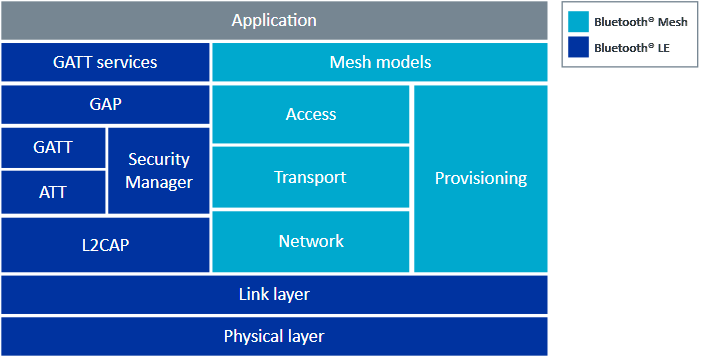
\includegraphics[width=1\textwidth]{chapter3/image/MeshStacknRF.png}
    \caption{Kiến trúc phân lớp của BLE Mesh và BLE \cite{nordic_mesh_architecture}}
    \label{fig:ble_mesh_stack_nrf}
\end{figure}

Lớp Network nằm ngay trên lớp Bearer, đảm nhiệm việc định địa chỉ và chuyển tiếp message trong mạng. Mỗi message được mã hóa bằng Network Key (NetKey) - một khóa được chia sẻ giữa tất cả các node trong cùng một subnet. Lớp này cũng quản lý cơ chế relay, cho phép các node trung gian chuyển tiếp message để mở rộng phạm vi phủ sóng của mạng. Để ngăn chặn việc message bị lặp vô hạn trong mạng, mỗi message được gán một giá trị TTL (Time To Live) giảm dần qua mỗi hop, và mỗi node duy trì một message cache để loại bỏ các message trùng lặp.

\begin{figure}[h!]
    \centering
    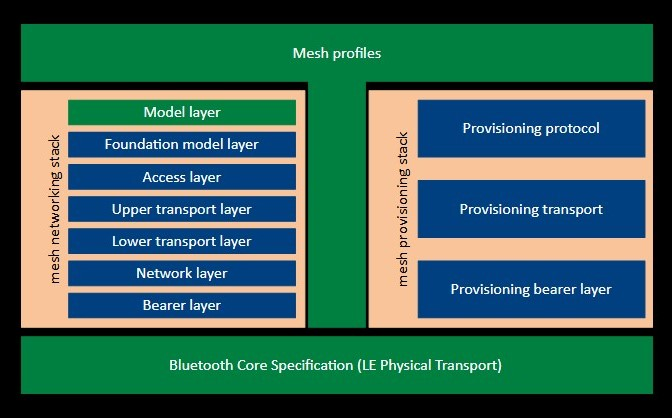
\includegraphics[width=1\textwidth]{chapter3/image/MeshStack.jpg}
    \caption{Kiến trúc phân lớp của BLE Mesh \cite{bluetooth_mesh_profile}}
    \label{fig:ble_mesh_stack}
\end{figure}

Lớp Lower Transport chịu trách nhiệm phân mảnh và tái hợp các message có kích thước lớn. Do giới hạn của BLE advertising packet (tối đa 31 bytes cho legacy advertising), các message có payload lớn hơn 11 bytes (sau khi trừ đi header) cần được chia thành nhiều segment. Lớp này cũng xử lý các message Friend và Low Power Node, cho phép các thiết bị tiết kiệm năng lượng tham gia vào mạng mesh.

Lớp Upper Transport cung cấp cơ chế mã hóa và xác thực ở mức application. Mỗi message được mã hóa bằng Application Key (AppKey), cho phép phân quyền truy cập đến các chức năng cụ thể của node. Một node có thể có nhiều AppKey khác nhau cho các ứng dụng khác nhau, ví dụ một AppKey cho điều khiển đèn và một AppKey khác cho điều khiển nhiệt độ.

Lớp Access định nghĩa cách các message được định dạng và gửi đến các Model trong node. Lớp này xử lý việc đóng gói opcode và payload thành Access PDU, và định tuyến các message đến đúng Model dựa trên opcode.

Lớp Model là lớp cao nhất, định nghĩa các chức năng và hành vi cụ thể của node. BLE Mesh SIG định nghĩa sẵn nhiều Standard Model cho các ứng dụng phổ biến như điều khiển đèn (Light Lightness Model), cảm biến (Sensor Model), và điều khiển nhiệt độ (Generic Level Model). Ngoài ra, các nhà phát triển có thể tạo Vendor Model để triển khai các chức năng tùy chỉnh theo yêu cầu riêng của ứng dụng.



\subsubsection{Cơ chế truyền tin trong BLE Mesh}

BLE Mesh sử dụng cơ chế Flooding để truyền message trong mạng. Khi một node gửi message, tất cả các node trong phạm vi phủ sóng đều nhận được message này. Các node có chức năng Relay sẽ chuyển tiếp message đến các node khác nếu node đó không phải địa chỉ đích, giúp message có thể đến được các node nằm ngoài phạm vi phủ sóng trực tiếp của node gửi.

Cơ chế Flooding có ưu điểm là đơn giản trong triển khai và không yêu cầu duy trì bảng định tuyến phức tạp. Tuy nhiên, nó cũng có nhược điểm là tạo ra nhiều traffic trong mạng, đặc biệt khi số lượng node lớn. Để giảm thiểu vấn đề này, BLE Mesh sử dụng một số kỹ thuật tối ưu gọi là managed flooding.

Thứ nhất, mỗi node duy trì một Message Cache để lưu trữ các message đã nhận gần đây. Khi nhận được một message, node kiểm tra xem message này đã có trong cache chưa. Nếu đã có, message sẽ bị loại bỏ ngay lập tức mà không được xử lý hay chuyển tiếp. Điều này ngăn chặn việc cùng một message bị xử lý nhiều lần hoặc lặp vô hạn trong mạng.

Thứ hai, mỗi message được gán một giá trị TTL (Time To Live) khi được tạo ra. Giá trị này giảm đi 1 mỗi khi message được chuyển tiếp qua một node. Khi TTL giảm về 0, message sẽ không được chuyển tiếp nữa. Cơ chế này giới hạn phạm vi lan truyền của message trong mạng, tránh tình trạng message bị broadcast không kiểm soát.

Thứ ba, BLE Mesh định nghĩa trạng thái Heartbeat trong Health Server Model để các node thông báo sự hiện diện của mình trong mạng. Heartbeat message được gửi định kỳ và chứa thông tin về số hop đến node gửi, giúp các node khác ước tính khoảng cách logic trong mạng.

\subsubsection{Provisioning và Security}

Provisioning là quá trình thêm một thiết bị mới vào mạng BLE Mesh. Quá trình này bao gồm việc trao đổi khóa bảo mật và gán địa chỉ unicast cho thiết bị. BLE Mesh sử dụng giao thức Elliptic Curve Diffie-Hellman (ECDH) để thiết lập kênh truyền an toàn trong quá trình provisioning, đảm bảo rằng các khóa không bị lộ ngay cả khi có kẻ tấn công nghe lén \cite{bluetooth_mesh_profile}.

BLE Mesh sử dụng mô hình bảo mật đa lớp với ba loại khóa chính. Network Key (NetKey) được chia sẻ giữa tất cả các node trong cùng một subnet và được sử dụng để mã hóa message ở lớp Network. Mỗi mạng mesh có thể có nhiều subnet với các NetKey khác nhau, cho phép phân vùng mạng theo các nhóm thiết bị. Application Key (AppKey) được sử dụng để mã hóa message ở lớp Upper Transport, cho phép phân quyền truy cập đến các chức năng cụ thể. Device Key (DevKey) là khóa duy nhất của mỗi thiết bị, được sử dụng trong quá trình configuration và firmware update.

Tất cả các message trong BLE Mesh đều được mã hóa và xác thực bằng AES-CCM với key size 128 bits. Điều này đảm bảo tính bảo mật (confidentiality), toàn vẹn (integrity), và xác thực (authenticity) của dữ liệu truyền trong mạng.

\subsubsection{Các loại Node trong BLE Mesh}

BLE Mesh định nghĩa nhiều vai trò (features) mà một node có thể đảm nhiệm, tùy thuộc vào khả năng phần cứng và yêu cầu của ứng dụng.

Relay Node là node có khả năng chuyển tiếp message đến các node khác trong mạng. Đây là tính năng quan trọng nhất của BLE Mesh, cho phép mở rộng phạm vi phủ sóng của mạng vượt xa giới hạn của một hop BLE. Không phải tất cả các node đều cần bật tính năng Relay; việc chọn node nào làm Relay phụ thuộc vào topology mạng và yêu cầu về độ phủ sóng.

Proxy Node cung cấp cầu nối GATT cho các thiết bị không hỗ trợ BLE Mesh advertising, như smartphone và tablet. Thông qua Proxy Node, các ứng dụng mobile có thể gửi và nhận message trong mạng mesh mà không cần hỗ trợ mesh ở mức firmware.

Friend Node và Low Power Node (LPN) tạo thành một cặp để hỗ trợ các thiết bị tiết kiệm năng lượng. LPN là các thiết bị chạy pin, hầu hết thời gian ở chế độ sleep để tiết kiệm năng lượng. Friend Node lưu trữ các message dành cho LPN và chuyển chúng khi LPN thức dậy và yêu cầu. Cơ chế này cho phép các thiết bị chạy pin tham gia vào mạng mesh mà vẫn duy trì thời gian hoạt động dài.

\subsubsection{Model trong BLE Mesh}

Model là đơn vị chức năng cơ bản trong BLE Mesh, định nghĩa hành vi và giao diện của một node. Mỗi Model bao gồm một tập hợp các State (trạng thái), Message (thông điệp), và Behavior (hành vi xử lý).

BLE Mesh SIG định nghĩa hai loại Model: SIG Model và Vendor Model. SIG Model là các model được chuẩn hóa bởi Bluetooth SIG với các Model ID từ 0x0000 đến 0xFFFF. Các SIG Model phổ biến bao gồm Generic OnOff Model cho điều khiển bật/tắt, Generic Level Model cho điều khiển mức (độ sáng, nhiệt độ), Light Lightness Model cho điều khiển đèn, và Sensor Model cho thu thập dữ liệu cảm biến. Việc sử dụng SIG Model đảm bảo tính tương thích giữa các thiết bị từ nhiều nhà sản xuất khác nhau.

Vendor Model cho phép các nhà phát triển tạo các model tùy chỉnh với chức năng riêng biệt. Mỗi Vendor Model được định danh bằng Company ID (được Bluetooth SIG cấp cho mỗi công ty) và Model ID do nhà phát triển định nghĩa. Vendor Model đặc biệt hữu ích khi cần triển khai các giao thức hoặc chức năng không được SIG Model hỗ trợ, như thuật toán định tuyến Gradient trong khóa luận này.

Mỗi Model hoạt động dựa trên cơ chế Publish-Subscribe. Node có thể publish message đến một địa chỉ (unicast, group, hoặc virtual address), và các node subscribe đến địa chỉ đó sẽ nhận được message. Cơ chế này cho phép thiết kế hệ thống linh hoạt, nơi một node có thể điều khiển nhiều node khác mà không cần biết trước danh sách các node đích.

